\chapter{Software Concept}

\label{ch: software}

In this chapter, the concept behind the software in development is presented. The entire software will be developed using Python, a powerful, simple and fast high-level programming language that has gained large space in various sectors of industry and academy. Its rise is due mainly to the enormous number of libraries and forums developed and maintained by the users. Some examples of libraries used in this project are \textit{numpy} (for scientific computing), \textit{matplotlib} (plotting library), \textit{Tkinter} and \textit{Qt} (Graphical User Interface toolkit). Python is also open-source, not requiring a paid software to code and most of its applications are free.

Although this project focus on using specific estimation methods and mathematical model for the DFIG problem, the software in development will not be specific to them. Instead, it will be generic and both model and method can be imported as packages. This will allow future users to use this application on different problems concerning parameter estimation. Also, comparison between method's performance and model's precision can be easily done with this software.

In order to improve the experience of users, a Graphical User Interface (GUI) is under development. It will provide an simple environment for all users, so they won't need to go through the code to change any settings. Instead, the settings will be done at the beginning of the process and follow a predefined order.

The starting window will display some information about the software and the parameter estimation process, as shown in Figure \ref{fig: init_pg}.

\begin{figure}[h]
	\caption{Representation of software starting window}
	\begin{center}
		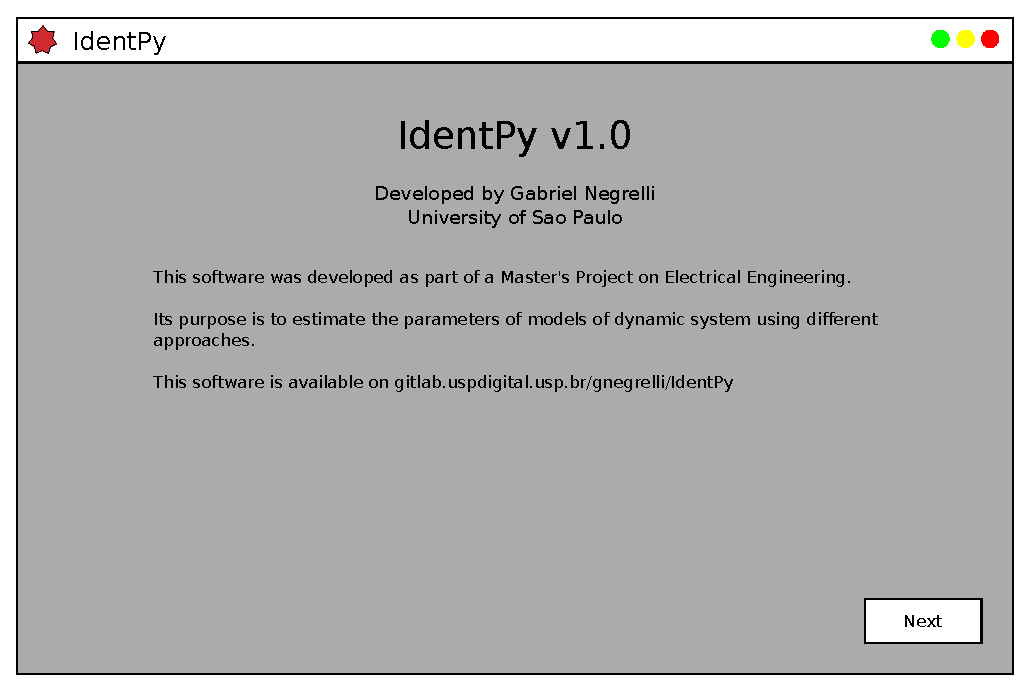
\includegraphics[scale=.5]{Images/Software_init_pg.eps}
	\end{center}
	\label{fig: init_pg}
\end{figure}

Next, the user will choose from a list which mathematical model will be employed, as depicted in Figure \ref{fig: pg1}. 

\begin{figure}[h]
	\caption{Representation of model selection window}
	\begin{center}
		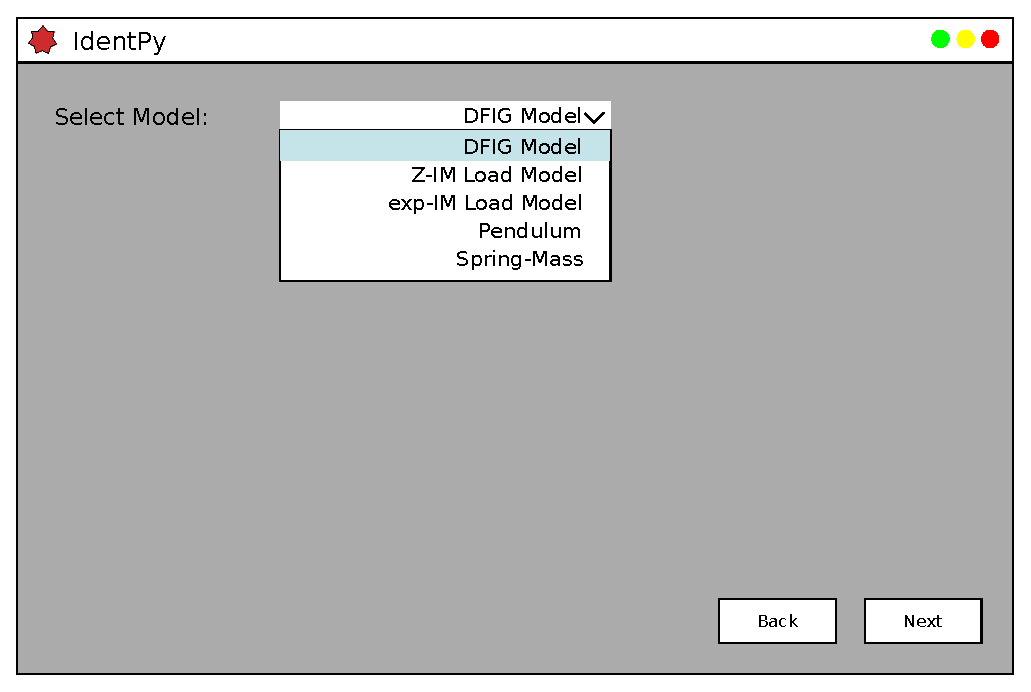
\includegraphics[scale=.5]{Images/Software_pg1.eps}
	\end{center}
	\label{fig: pg1}
\end{figure}

After that, a list of identification methods will be presented and the user will be able to pick up to two methods, as displayed in Figure \ref{fig: pg2}.

\begin{figure}[h]
	\caption{Representation of method selection window}
	\begin{center}
		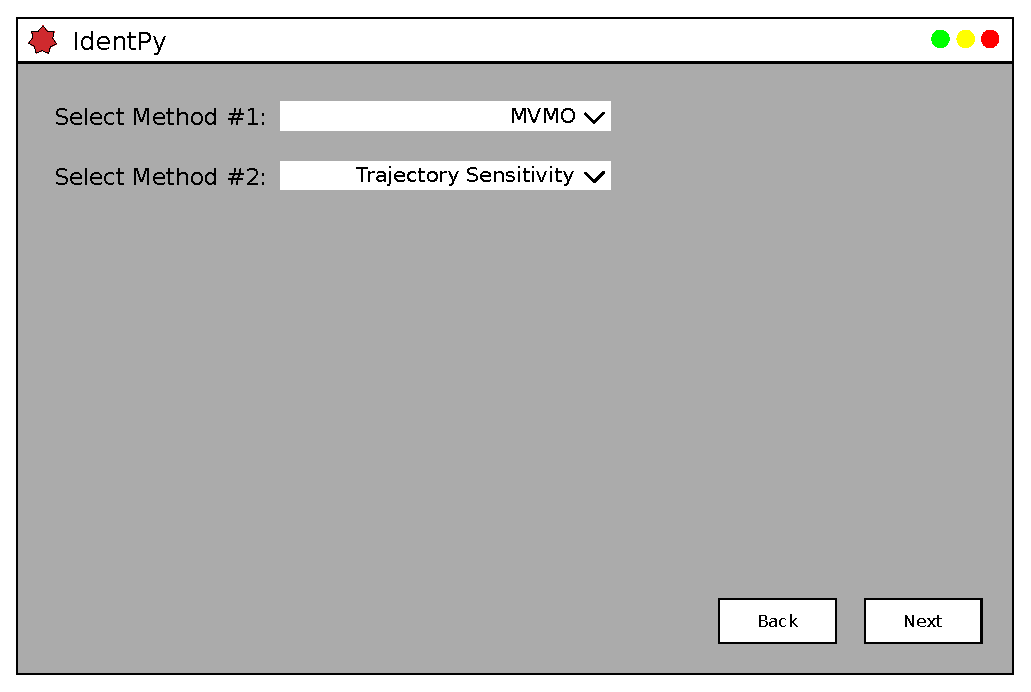
\includegraphics[scale=.5]{Images/Software_pg2.eps}
	\end{center}
	\label{fig: pg2}
\end{figure}


The settings of the chosen methods will done on the following windows and, finally, the user will enter the file containing the real system data and point out which data will be used as inputs and outputs. These steps are shown in Figures \ref{fig: pg3} and \ref{fig: pg4}, respectively.

\begin{figure}[h]
	\caption{Representation of method setting window}
	\begin{center}
		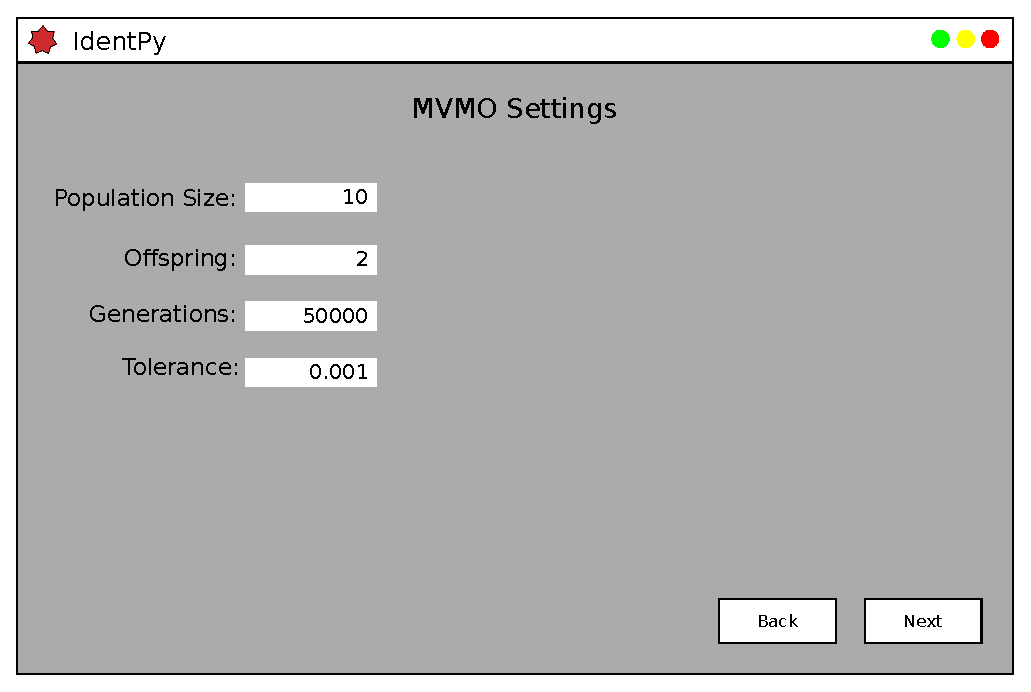
\includegraphics[scale=.5]{Images/Software_pg3.eps}
	\end{center}
	\label{fig: pg3}
\end{figure}

\begin{figure}[h]
	\caption{Representation of file selection window}
	\begin{center}
		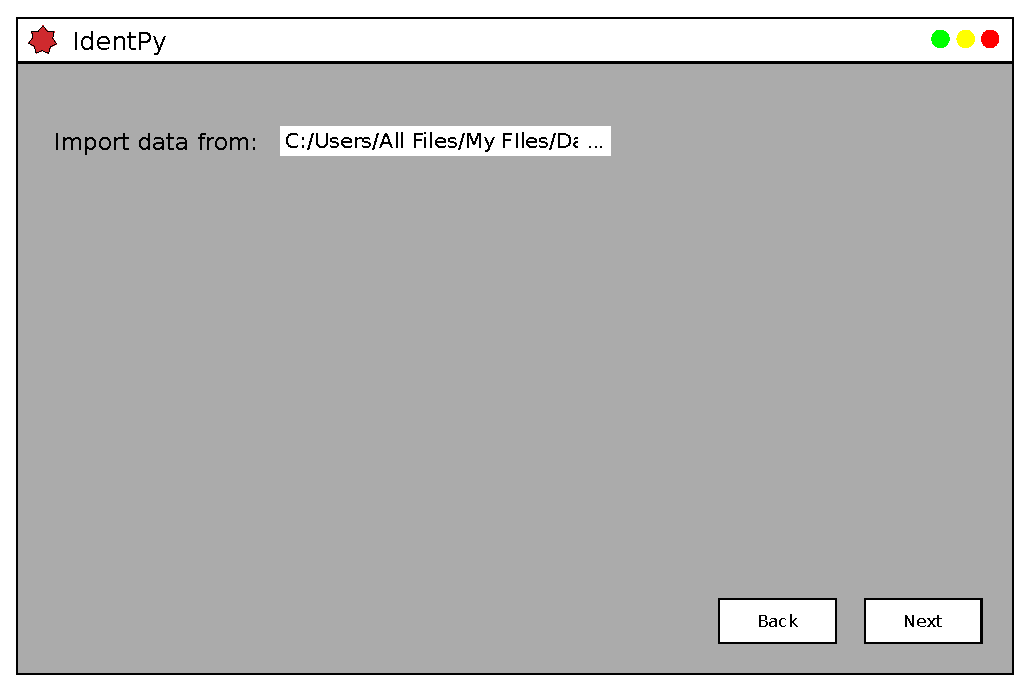
\includegraphics[scale=.5]{Images/Software_pg4.eps}
	\end{center}
	\label{fig: pg4}
\end{figure}

With all set, the estimation process will start and, at its end, a report will display the estimated parameters and the comparison between real system and model behaviours. The final view is represented in Figure \ref{fig: final_pg}

\begin{figure}[h]
	\caption{Representation of report window}
	\begin{center}
		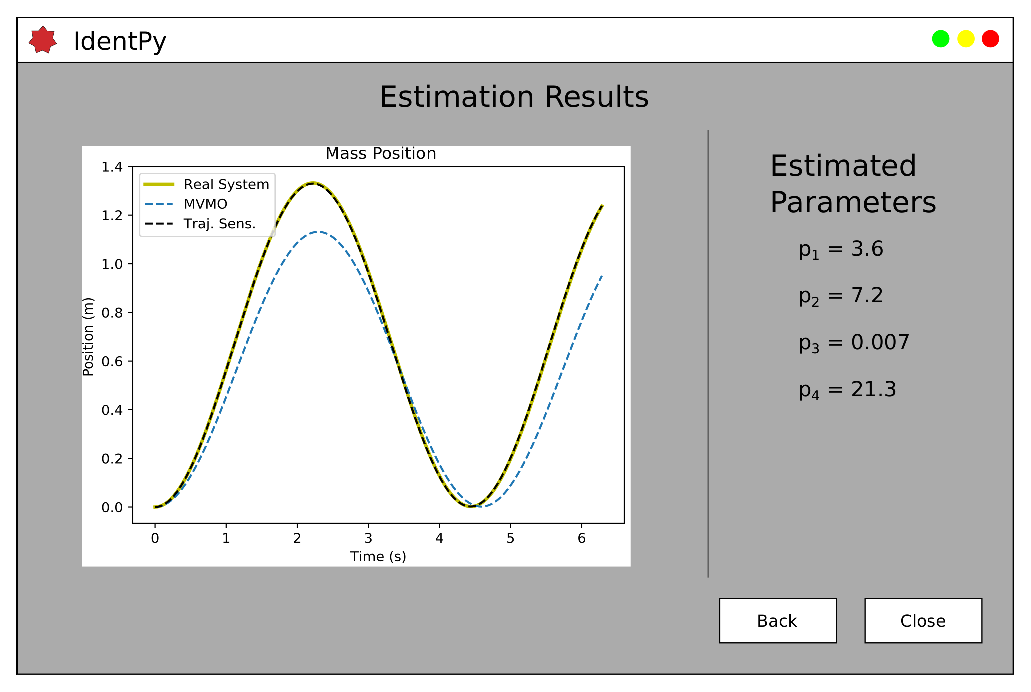
\includegraphics[scale=.5]{Images/Software_final_pg.eps}
	\end{center}
	\label{fig: final_pg}
\end{figure}

The order presented is not definitive and may change throughout the project if needed. However, all the steps discussed are core to the estimation process and cannot be discarded. Also, some other steps may be included in order to improve the software performance.